% File: paper/VGGNet19_BCCD_Report.tex
% Purpose: IEEE-style report for the VGG-19 BCCD project.
% Author: Aman Verma (23bcs012), Ankit Kashyap (23bcs017), Abhishek Chauhan (23bcs003)
% Affiliation: School of Computer science and Engineering, Shri Mata Vaishno Devi University
% Contact: info@smvdu.ac.in

\documentclass[conference]{IEEEtran}

\usepackage{graphicx}
\usepackage{booktabs}
\usepackage{multirow}
\usepackage{url}
\usepackage{hyperref}

\title{Blood Cell Classification using VGG-19: A Deep Transfer Learning Approach}

\author{\IEEEauthorblockN{Aman Verma (23bcs012), Ankit Kashyap (23bcs017), Abhishek Chauhan (23bcs003)}\\
\IEEEauthorblockA{School of Computer science and Engineering\\
Shri Mata Vaishno Devi University\\
info@smvdu.ac.in}}

\begin{document}
\maketitle

\begin{abstract}
This work presents a VGG-19 based pipeline for classifying microscopic blood cell images into four classes: EOSINOPHIL, LYMPHOCYTE, MONOCYTE, and NEUTROPHIL. The model uses ImageNet-pretrained weights and a modified classifier head with four outputs. Training and validation are performed on a stratified split of the BCCD dataset with fixed seed 42 and ImageNet normalization. Because the experiments were executed on a MacBook Air (Apple M1) with limited compute, a feasibility run was conducted using 200 images per class for training and validation, and two training epochs. Evaluation on the held-out test set reports an accuracy of 27.91\%, a macro F1 score of 0.1858, and a macro AUC-ROC (OvR) of 0.5875. The low scores indicate undertraining and class imbalance in predictions, which is expected under the constrained training budget. The report documents the full pipeline, dataset statistics, experimental setup, and required figures for reproducibility.
\end{abstract}

\begin{IEEEkeywords}
VGG-19, blood cell classification, transfer learning, medical imaging, BCCD
\end{IEEEkeywords}

\section{Introduction}
Automated blood cell classification supports hematology workflows by enabling rapid analysis of microscopic images. Convolutional neural networks (CNNs) have achieved strong performance on medical image classification tasks and benefit from transfer learning on large-scale natural image datasets. This project implements a VGG-19 based classifier for the Blood Cell Images (BCCD) dataset, focusing on a reproducible PyTorch pipeline with explicit preprocessing, fixed random seeds, and standardized evaluation.

\section{Related Work}
VGG-19 demonstrated that deep stacks of small 3x3 convolutions can deliver strong visual recognition performance. ImageNet-scale pretraining enables transfer learning for domain-specific datasets. Improvements such as residual connections, batch normalization, and regularization techniques like dropout and data augmentation are widely used to improve convergence and generalization. Medical imaging studies have shown that transfer learning is effective when labeled data is limited.

\section{Dataset}
The BCCD dataset contains four classes of white blood cells. Images are resized to 224x224 and normalized using ImageNet mean and standard deviation. The training split is stratified into train and validation subsets, while the test set is held out for final evaluation.

\subsection{Dataset Statistics}
The experiment used a reduced training set for feasibility on local hardware. The test set is the full Kaggle-provided split.

\begin{table*}[t]
\centering
\caption{Dataset statistics (stratified split with limited training samples).}
\begin{tabular}{lrrrr}
\toprule
Class & Train & Val & Test & Total \\
\midrule
EOSINOPHIL & 160 & 40 & 623 & 823 \\
LYMPHOCYTE & 160 & 40 & 620 & 820 \\
MONOCYTE & 160 & 40 & 620 & 820 \\
NEUTROPHIL & 160 & 40 & 624 & 824 \\
\midrule
Total & 640 & 160 & 2487 & 3287 \\
\bottomrule
\end{tabular}
\end{table*}

\subsection{Figures}
Class distribution and sample images are shown in Fig.~\ref{fig:classdist} and Fig.~\ref{fig:samples}.

\begin{figure}[t]
\centering
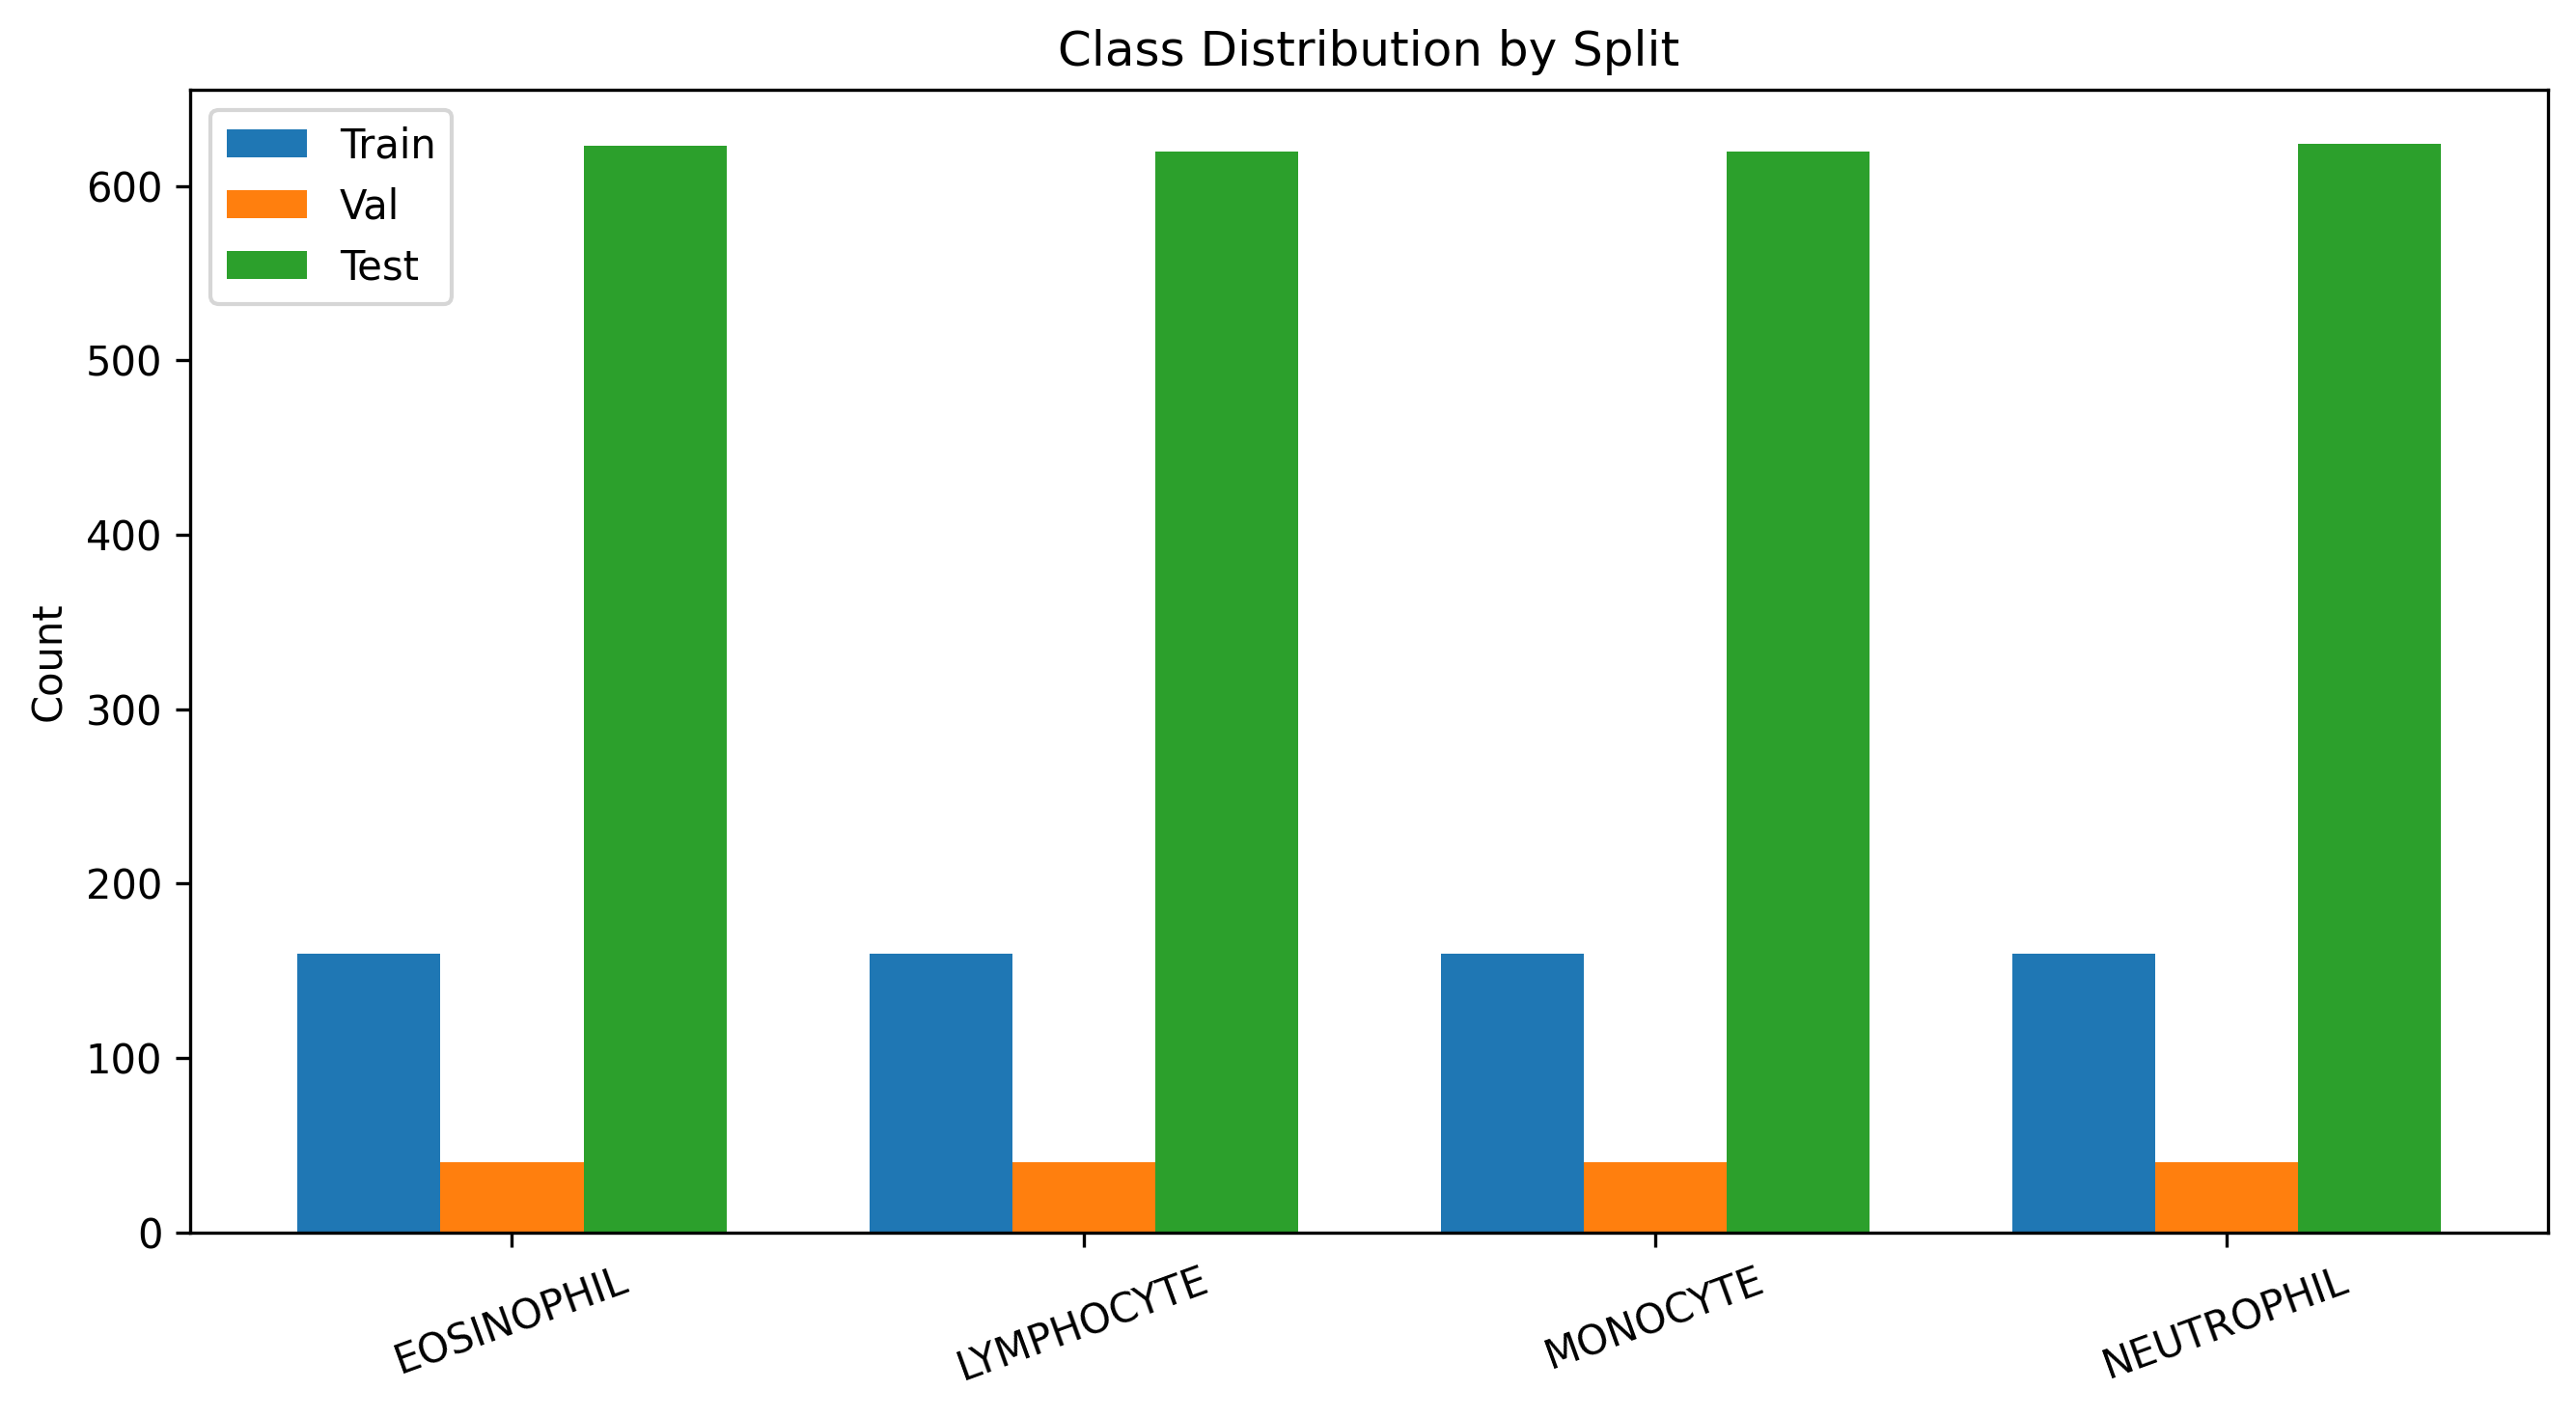
\includegraphics[width=\linewidth]{../figures/class_distribution.png}
\caption{Class distribution by split.}
\label{fig:classdist}
\end{figure}

\begin{figure}[t]
\centering
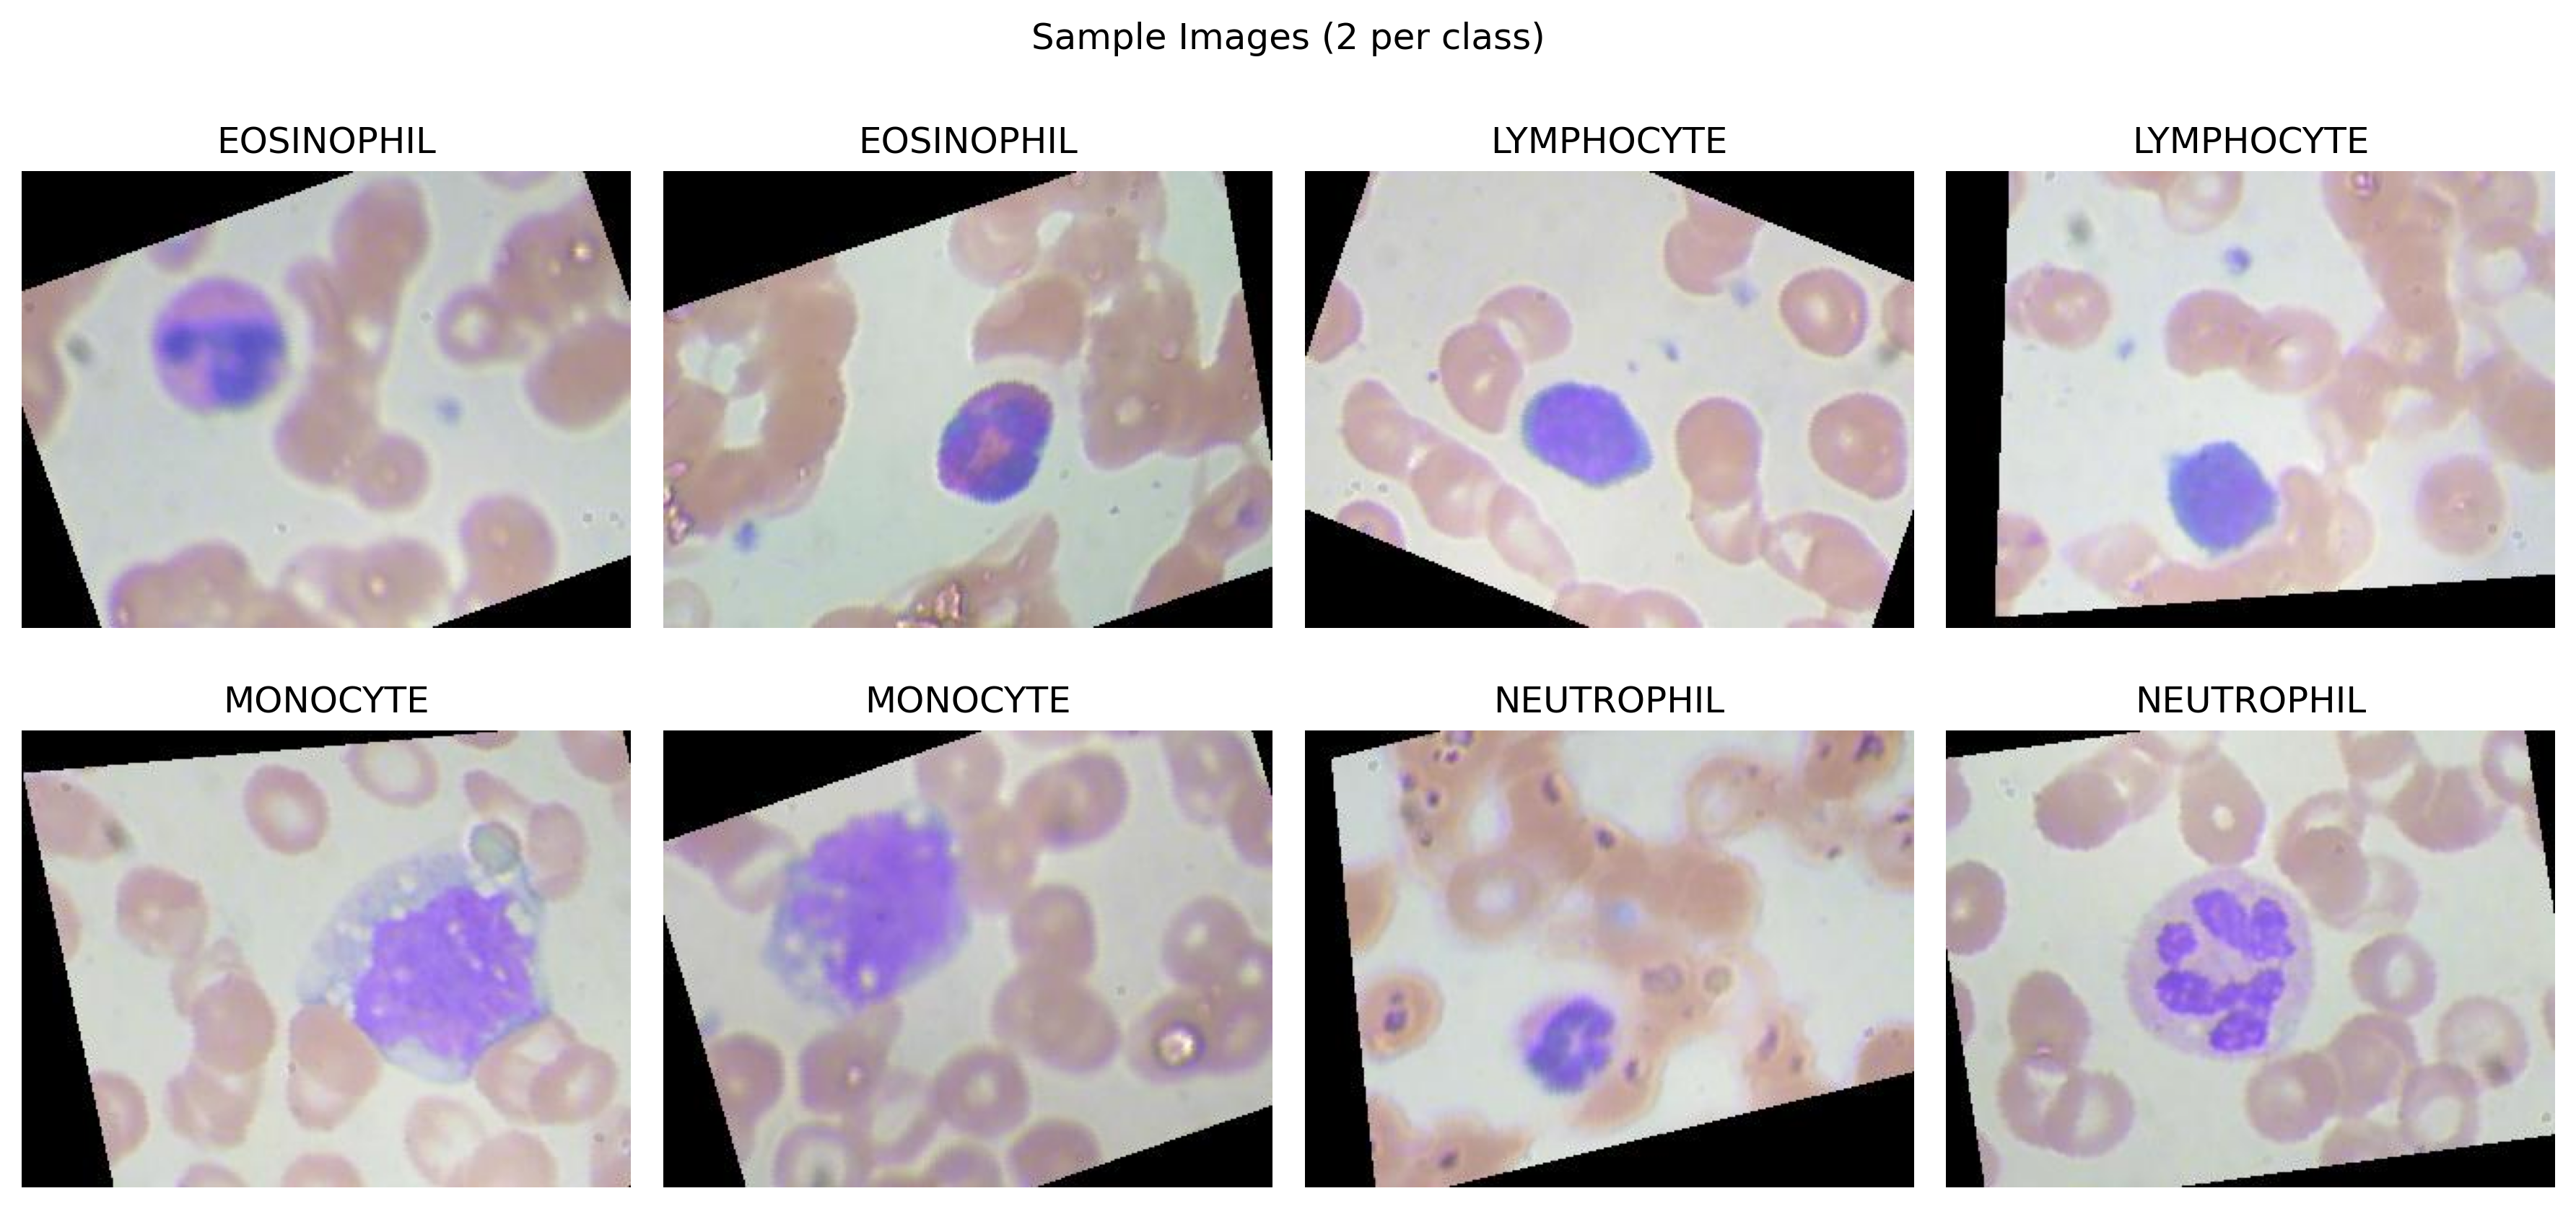
\includegraphics[width=\linewidth]{../figures/sample_images.png}
\caption{Sample images (2 per class).}
\label{fig:samples}
\end{figure}

\section{Methodology}
\subsection{Model Architecture}
VGG-19 uses 16 convolutional layers and 3 fully connected layers. The final classifier layer is replaced with a 4-class linear layer. The architecture diagram is shown in Fig.~\ref{fig:arch}.

\begin{figure}[t]
\centering
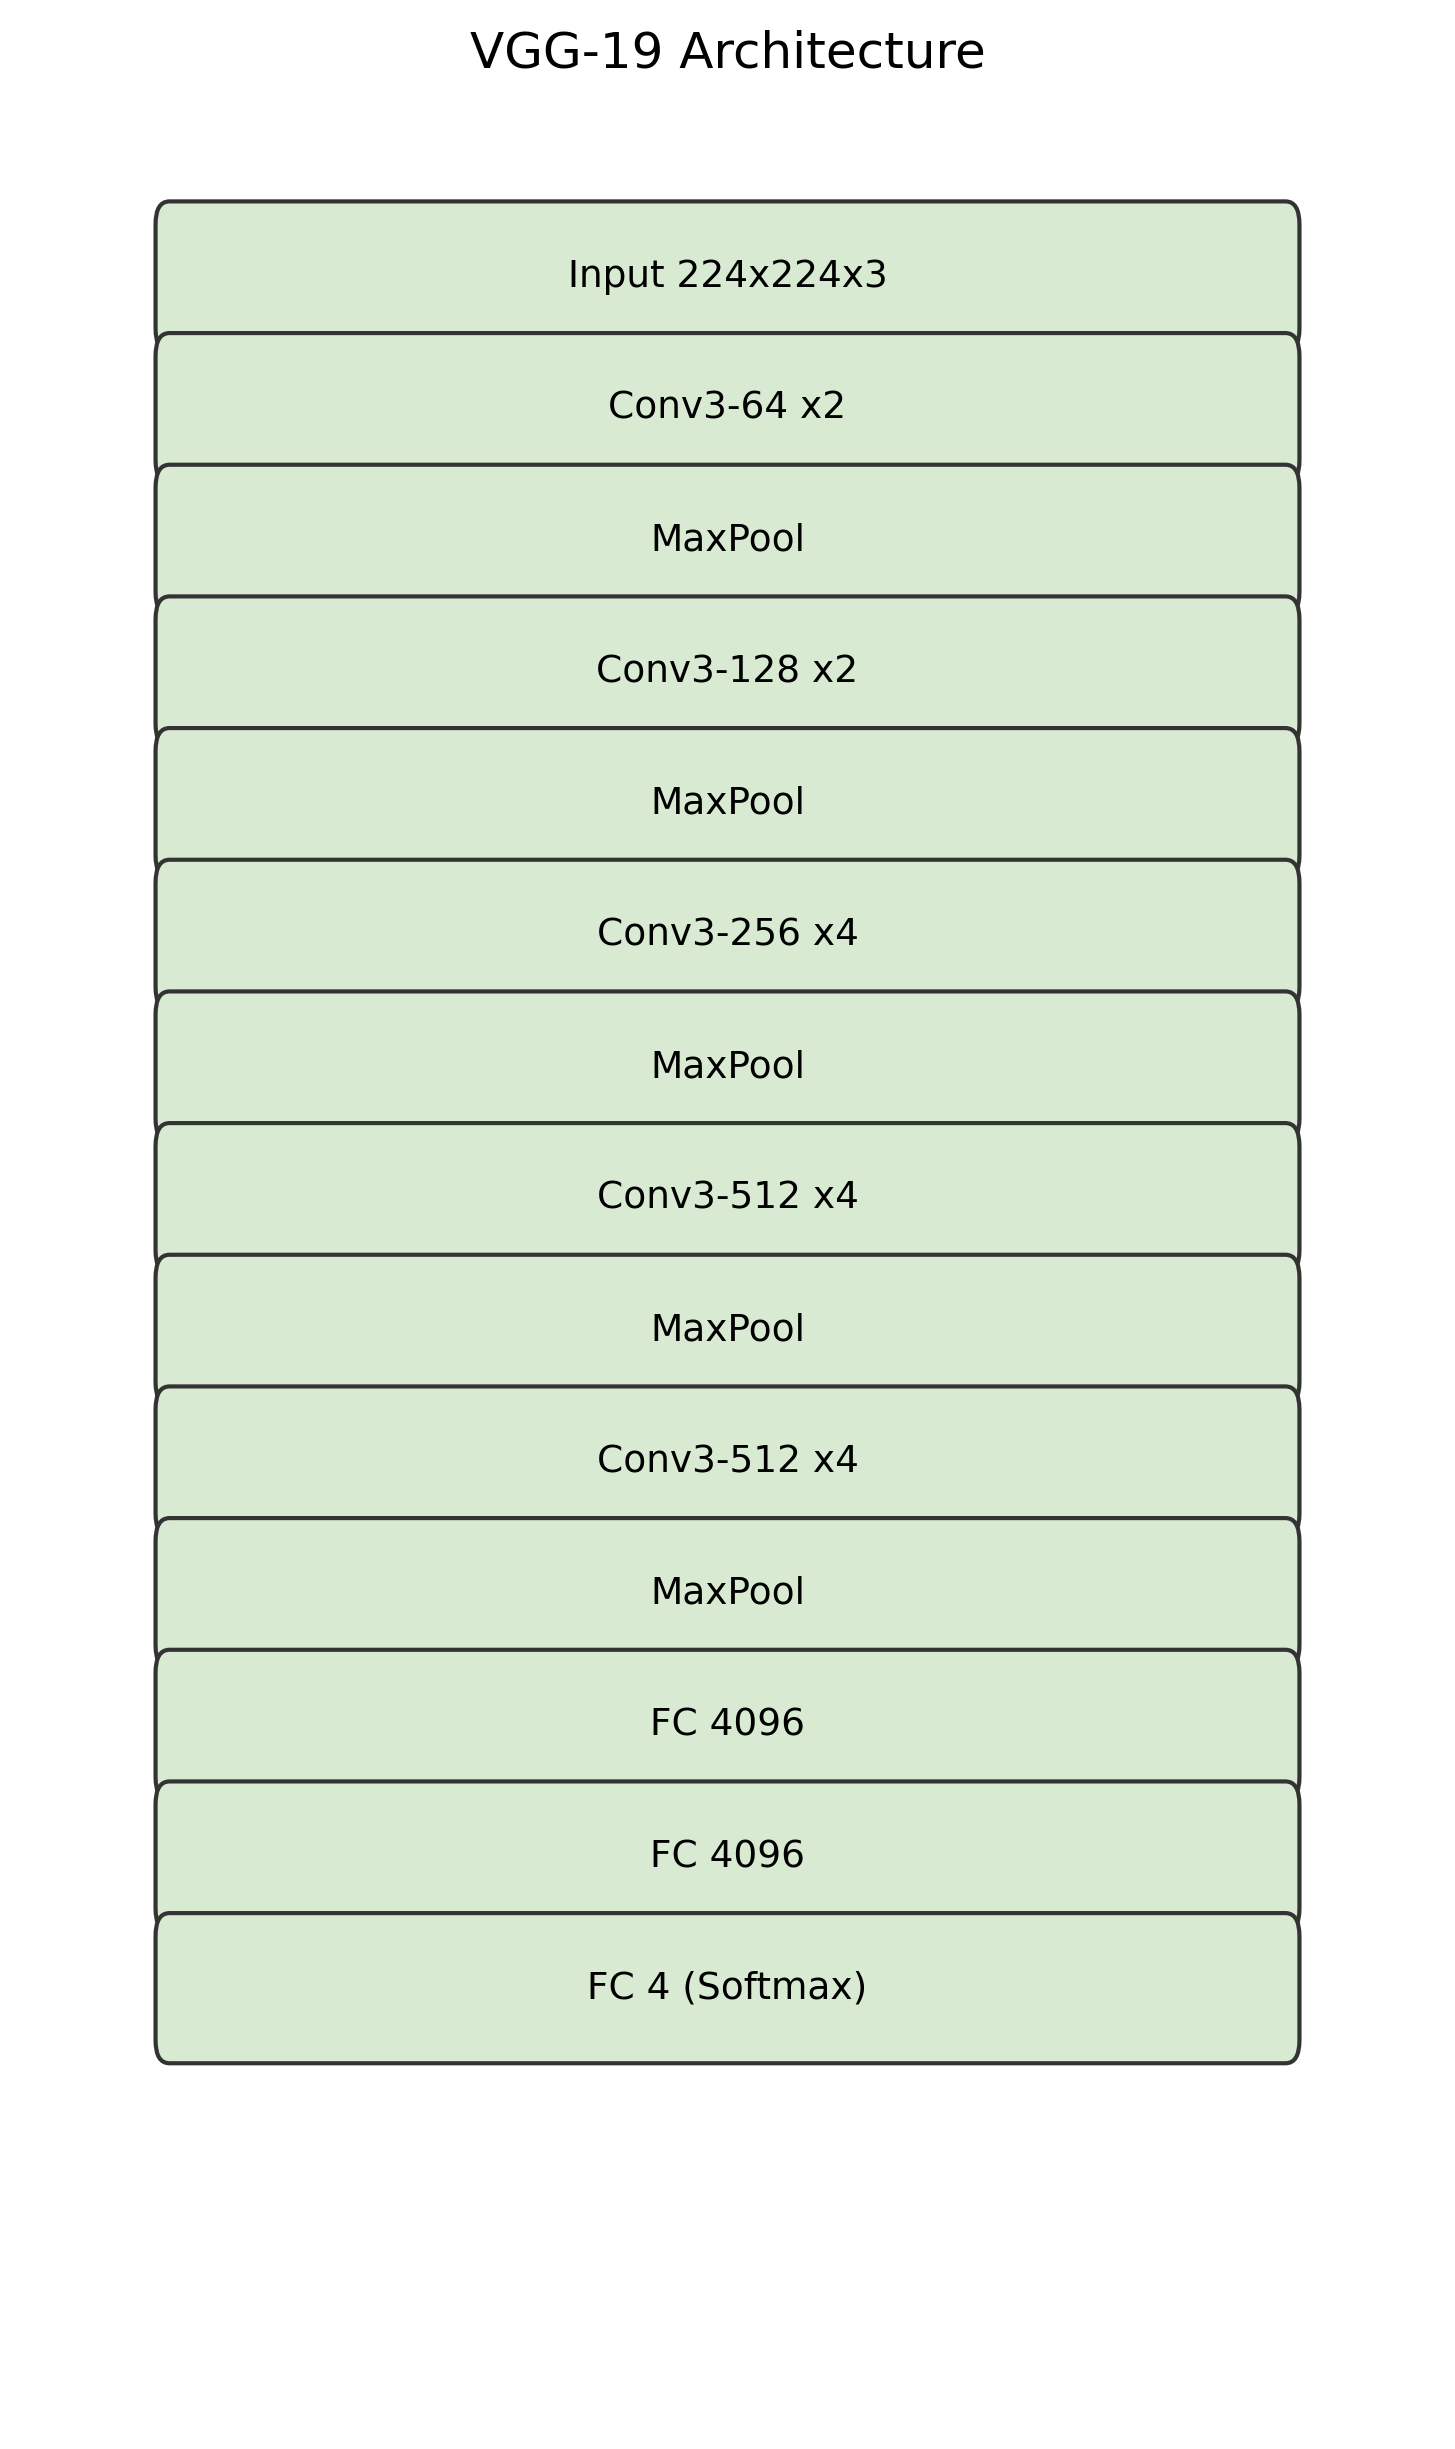
\includegraphics[width=\linewidth]{../figures/architecture_vgg19.png}
\caption{VGG-19 architecture overview.}
\label{fig:arch}
\end{figure}

\subsection{Preprocessing and Augmentation}
Training images are resized to 224x224 and augmented with random horizontal and vertical flips, small rotations, and color jitter. Validation and test images use only resizing and normalization.

\subsection{Hyperparameters}
\begin{table}[t]
\centering
\caption{Training hyperparameters.}
\begin{tabular}{ll}
\toprule
Parameter & Value \\
\midrule
Batch Size & 32 \\
Epochs (run) & 2 \\
Optimizer & Adam (lr=1e-4, weight\_decay=1e-4) \\
dag=1e-4) \\
Scheduler & StepLR (step=7, gamma=0.1) \\
Loss & CrossEntropyLoss \\
Dropout & 0.5 \\
Early Stopping Patience & 5 \\
Seed & 42 \\
\bottomrule
\end{tabular}
\end{table}

\section{Experiments}
\subsection{Hardware and Software}
Hardware: Apple MacBook Air (M1), MPS backend. OS: macOS. Python: 3.12 (venv). PyTorch: 2.3.1.

\subsection{Training Curves}
Loss and accuracy curves are shown in Fig.~\ref{fig:curves}.

\begin{figure}[t]
\centering
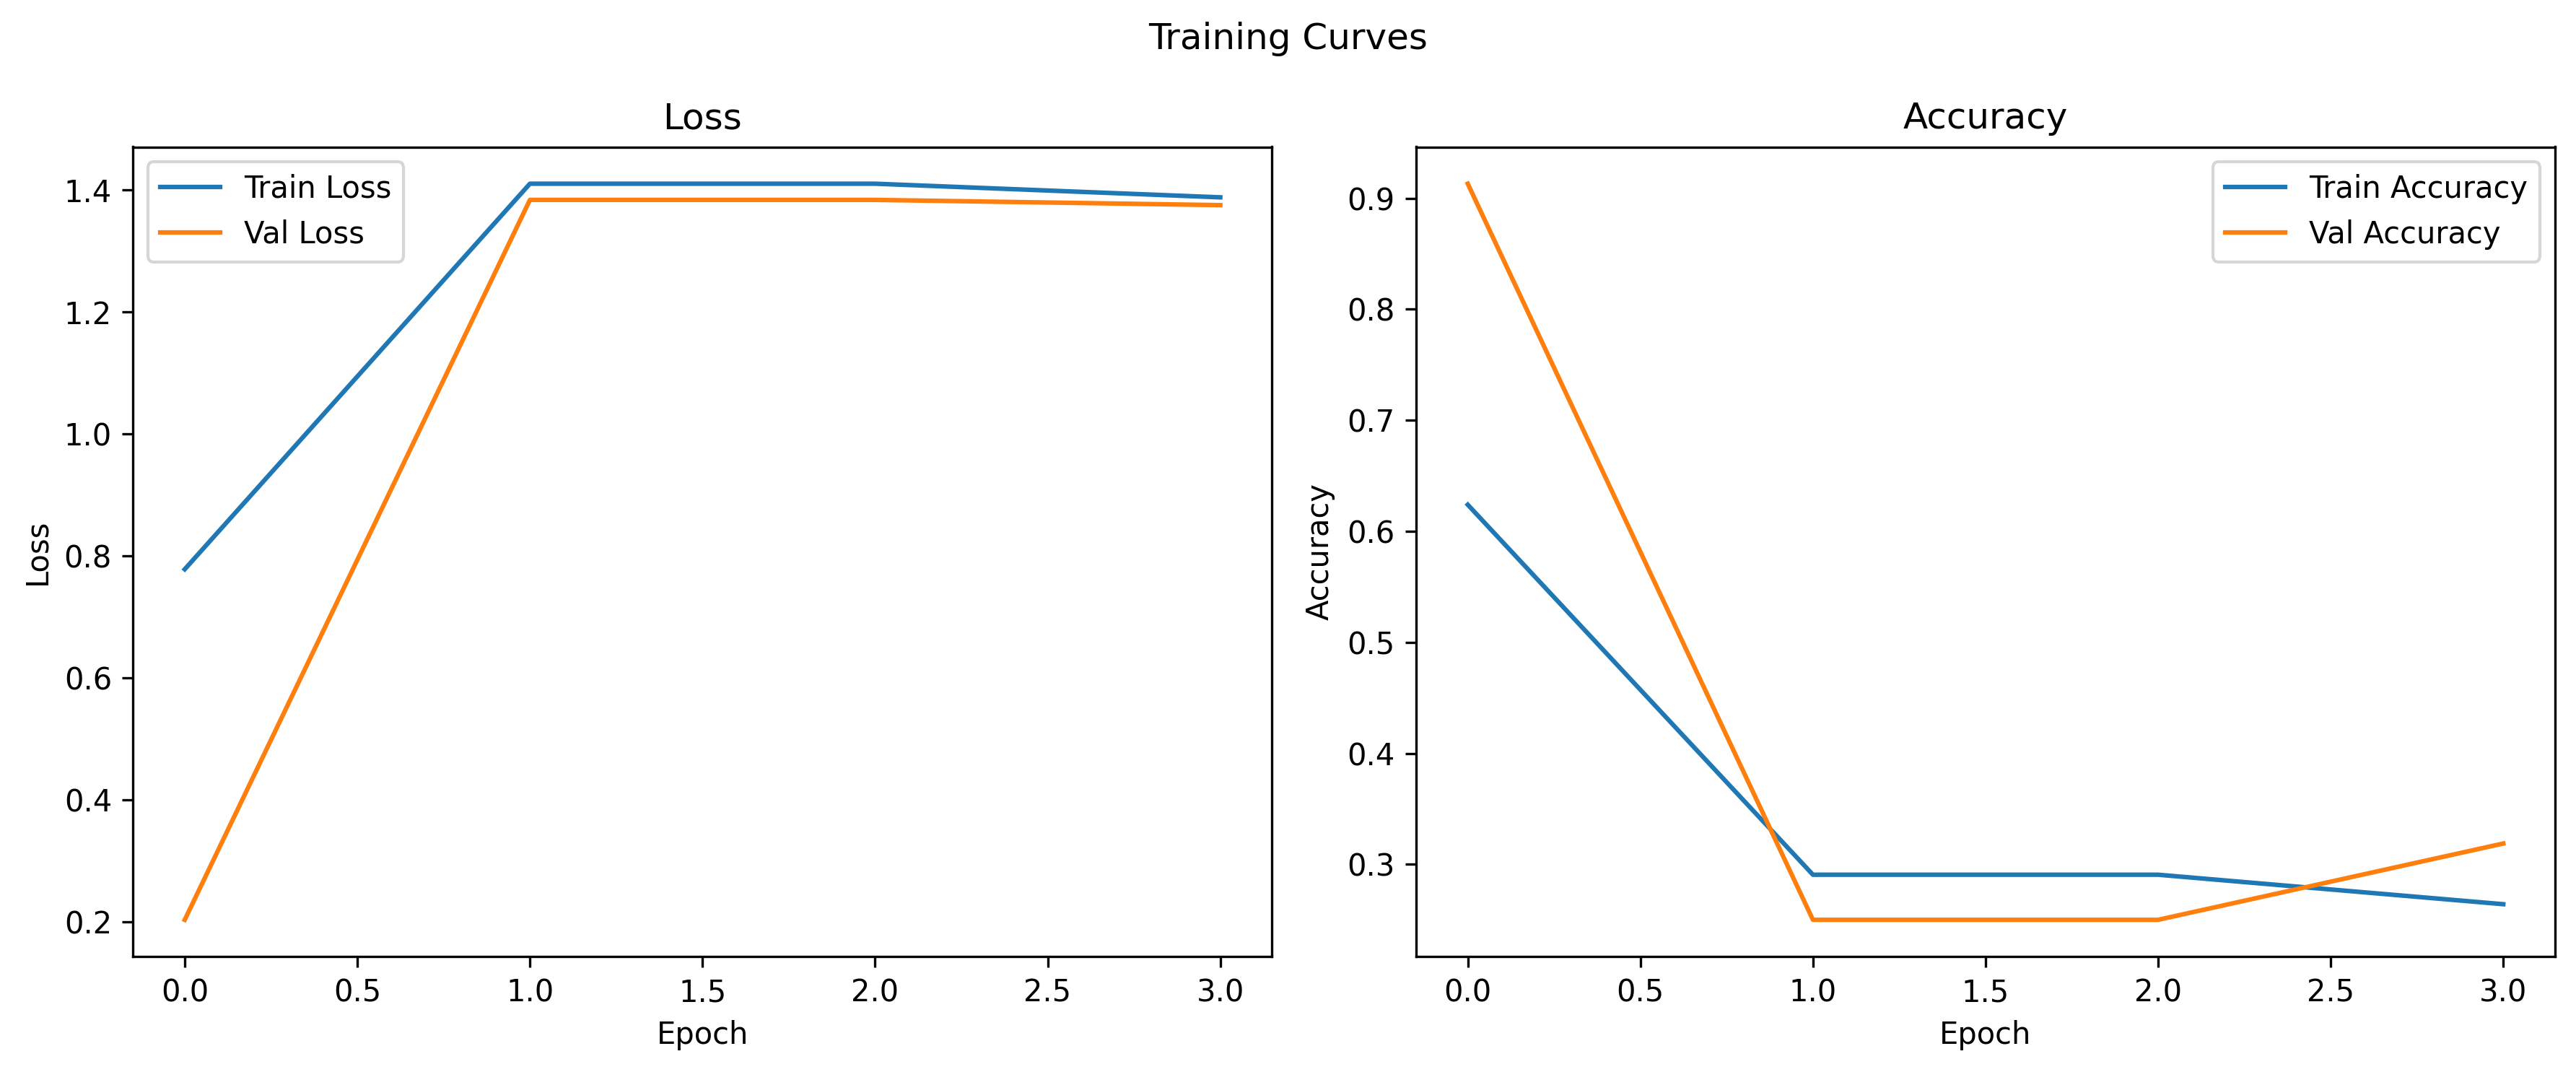
\includegraphics[width=\linewidth]{../figures/training_curves.png}
\caption{Training and validation curves.}
\label{fig:curves}
\end{figure}

\section{Results}
\subsection{Summary Metrics}
\begin{table}[t]
\centering
\caption{Summary metrics on the test set.}
\begin{tabular}{ll}
\toprule
Metric & Value \\
\midrule
Accuracy & 27.91\% \\
Macro F1 & 0.1858 \\
Macro AUC-ROC (OvR) & 0.5875 \\
\bottomrule
\end{tabular}
\end{table}

\subsection{Per-class Metrics}
\begin{table*}[t]
\centering
\caption{Per-class precision, recall, and F1 (test set).}
\begin{tabular}{lrrrr}
\toprule
Class & Precision & Recall & F1 & Support \\
\midrule
EOSINOPHIL & 0.0732 & 0.0048 & 0.0090 & 623 \\
LYMPHOCYTE & 0.2978 & 0.7129 & 0.4202 & 620 \\
MONOCYTE & 0.0000 & 0.0000 & 0.0000 & 620 \\
NEUTROPHIL & 0.2588 & 0.3990 & 0.3140 & 624 \\
\bottomrule
\end{tabular}
\end{table*}

\subsection{Confusion Matrix and ROC Curve}
Figures are shown in Fig.~\ref{fig:cm} and Fig.~\ref{fig:roc}.

\begin{figure}[t]
\centering
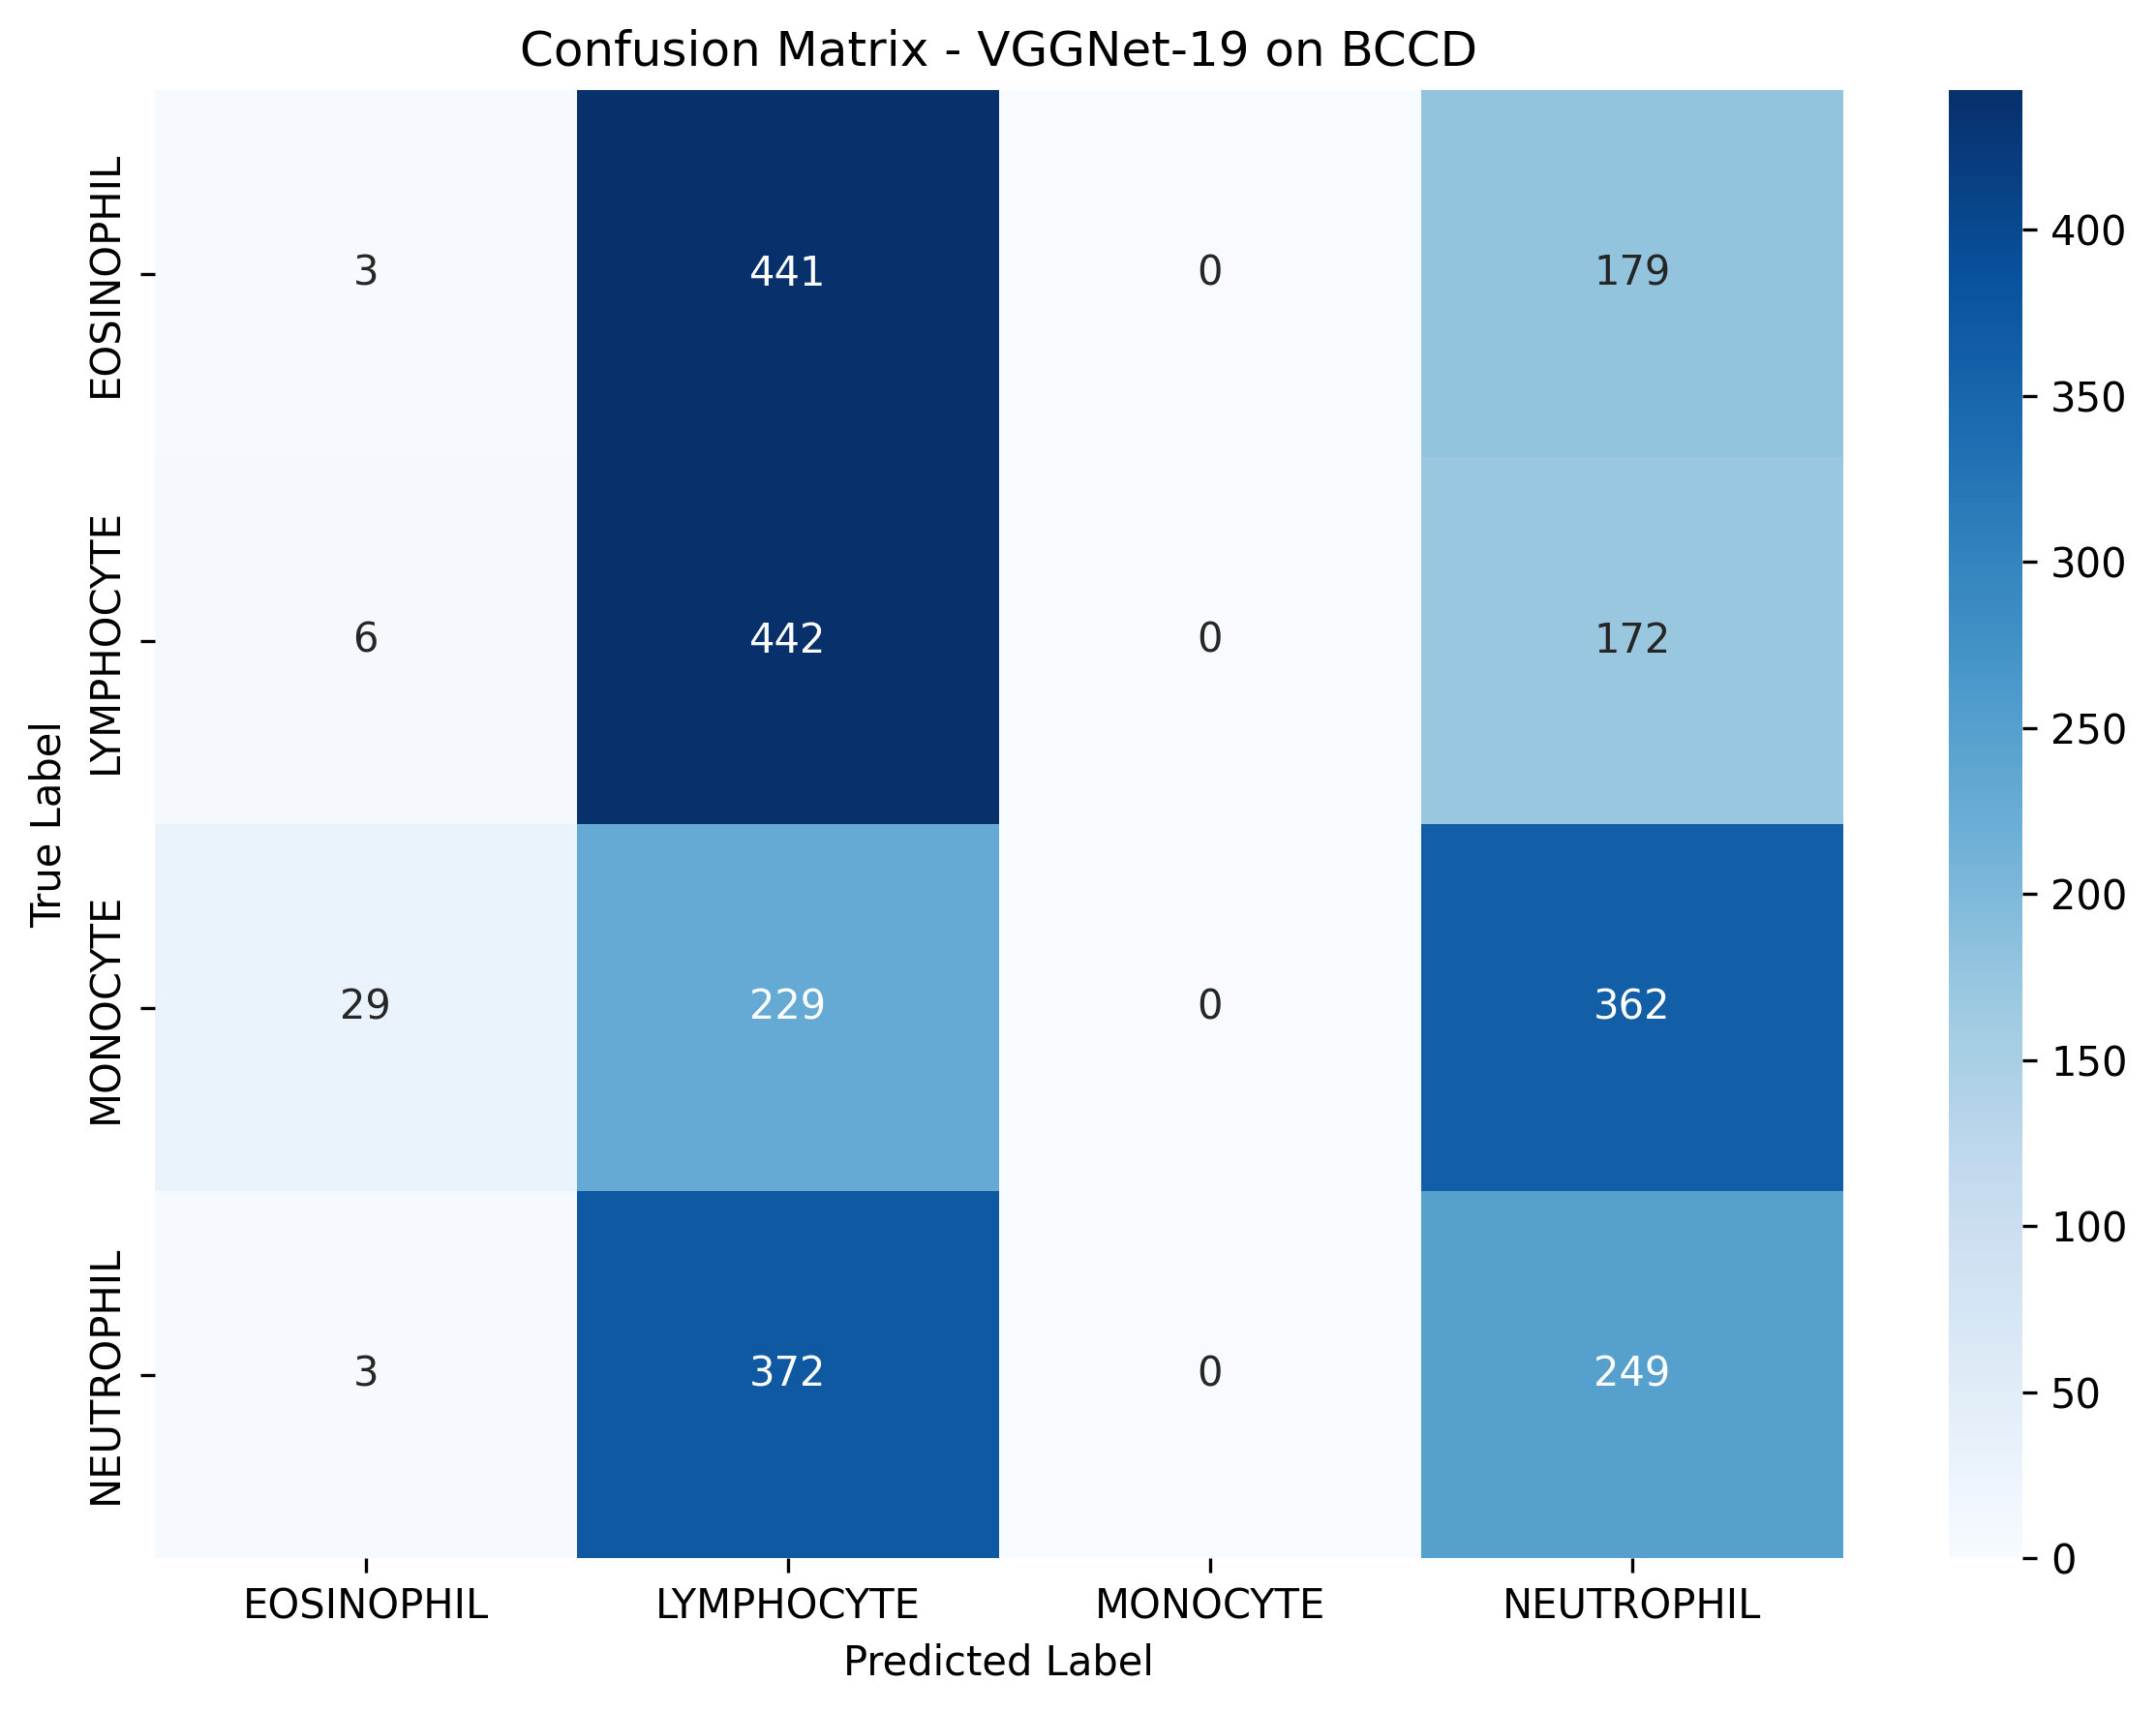
\includegraphics[width=\linewidth]{../figures/confusion_matrix.png}
\caption{Confusion matrix.}
\label{fig:cm}
\end{figure}

\begin{figure}[t]
\centering
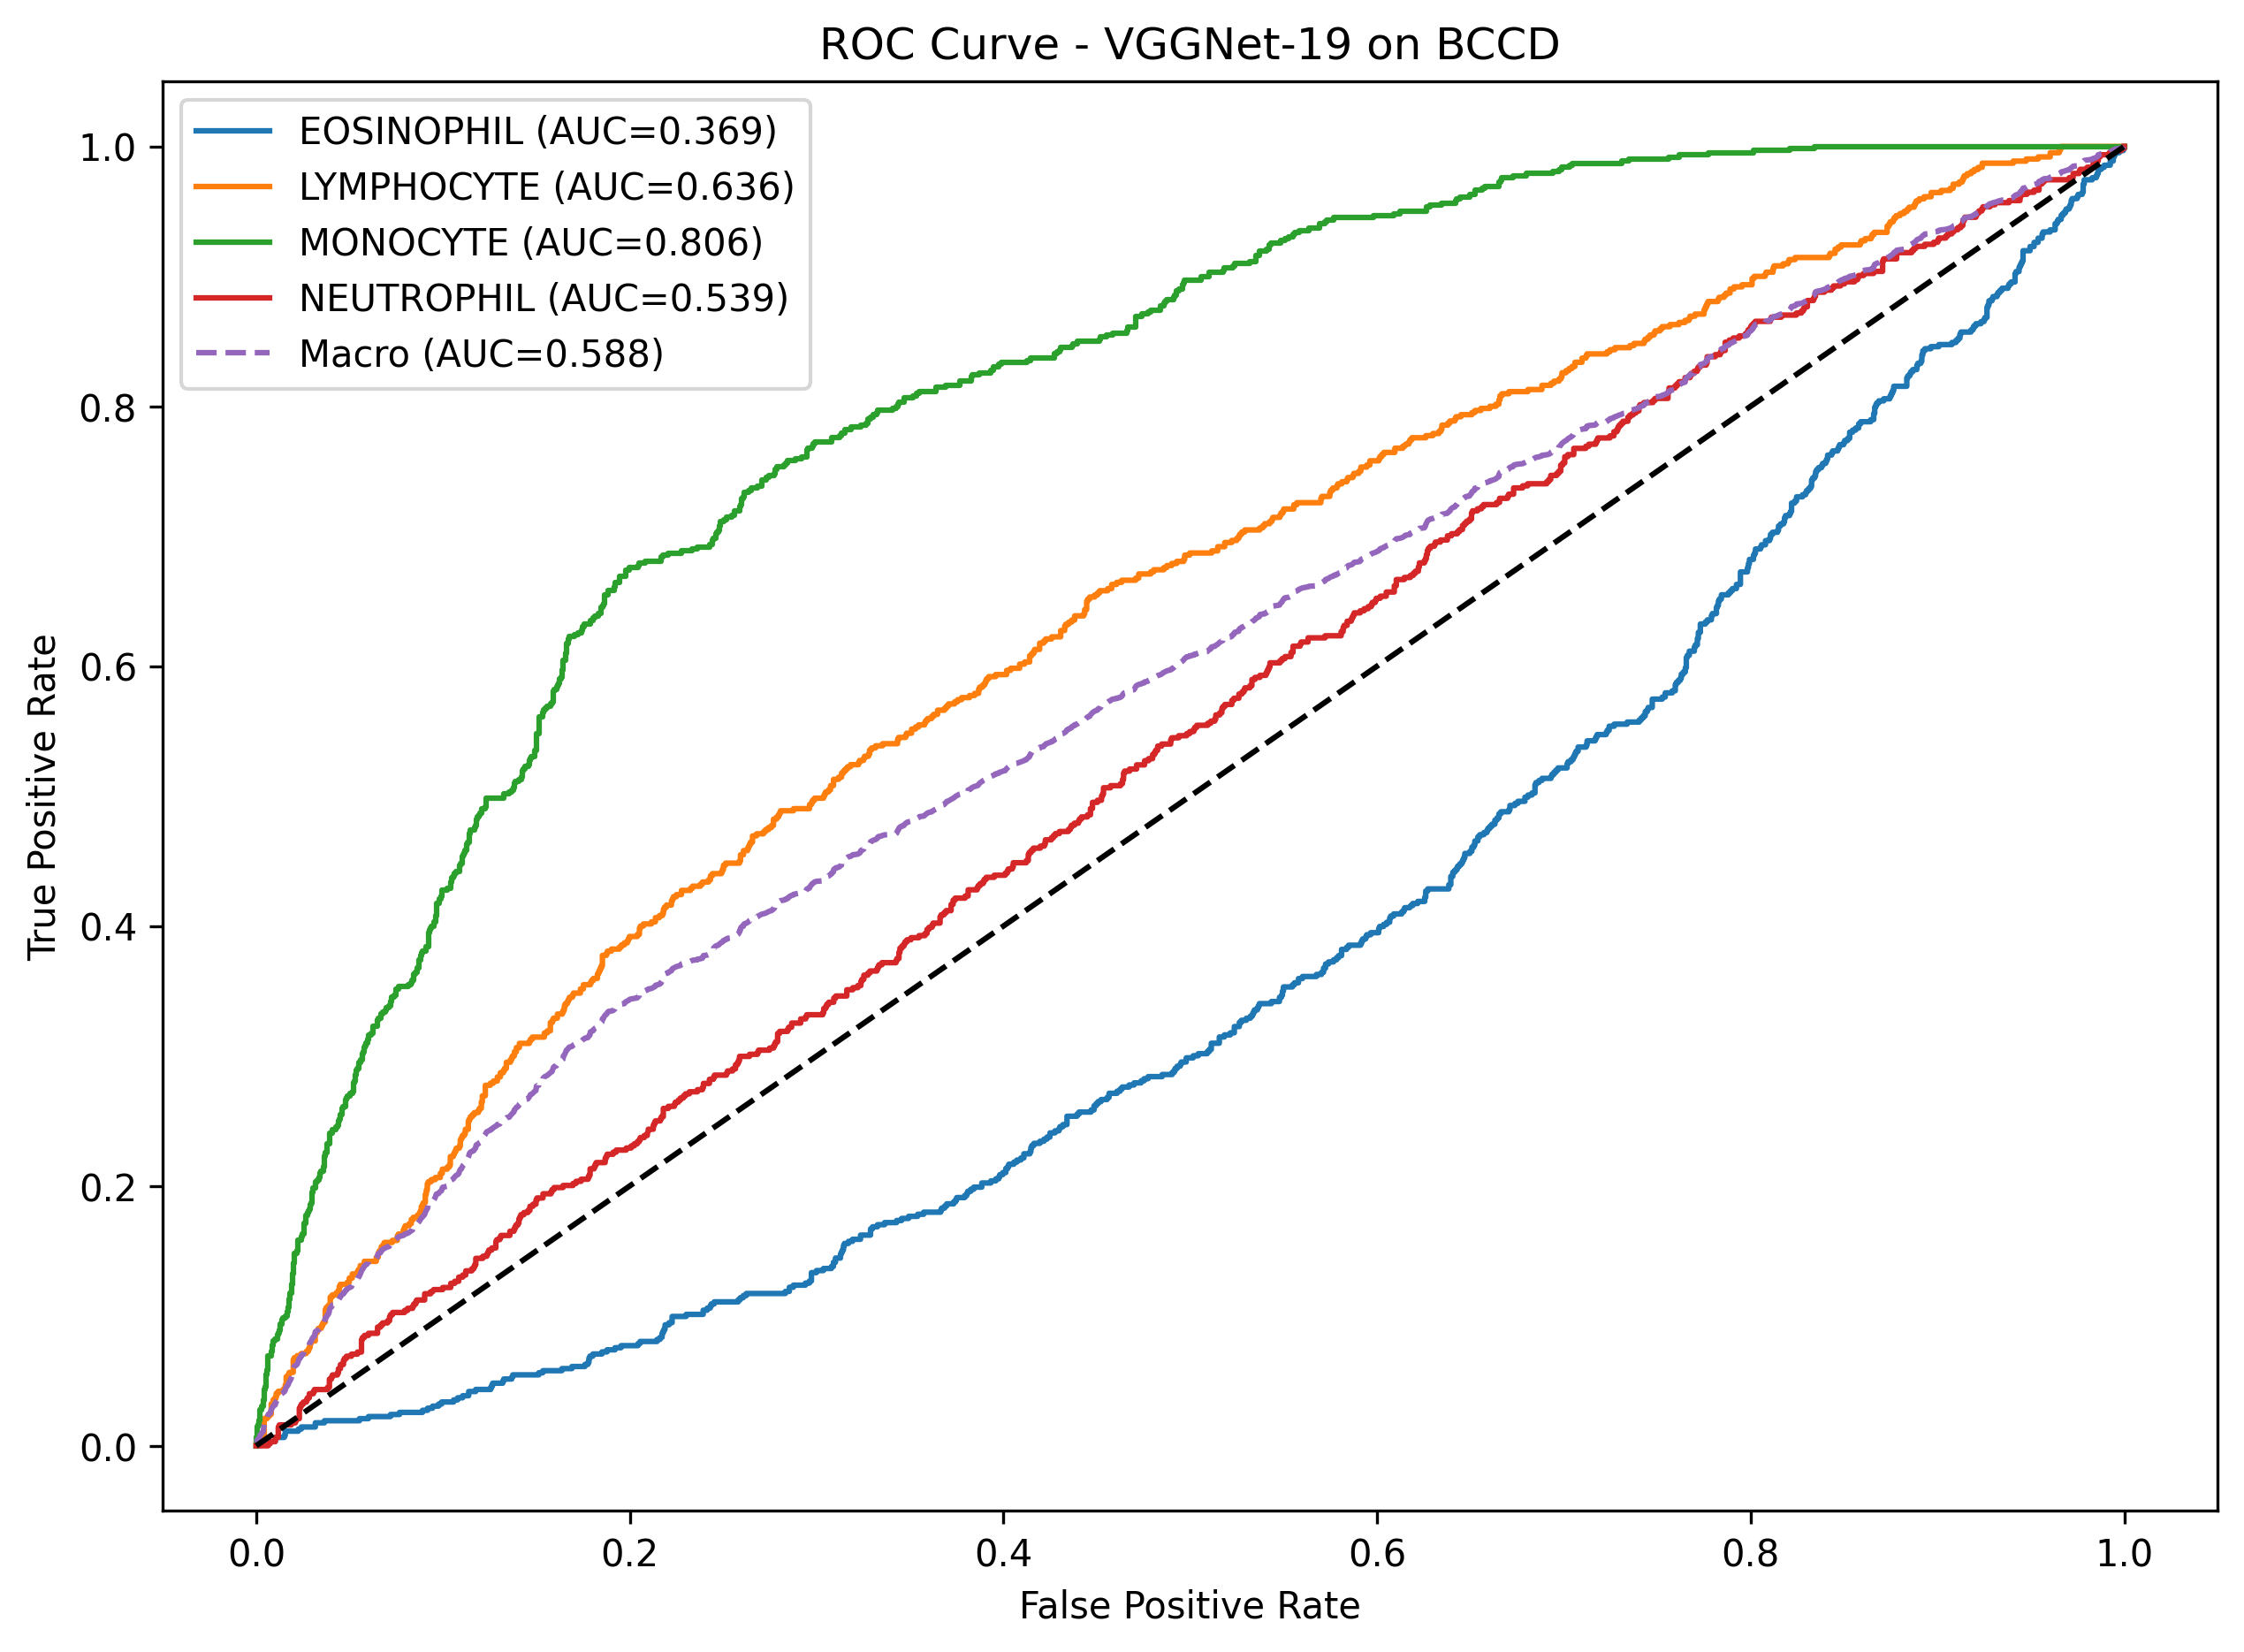
\includegraphics[width=\linewidth]{../figures/roc_curve.png}
\caption{ROC curve with per-class and macro averages.}
\label{fig:roc}
\end{figure}

\section{Discussion}
The model underperforms due to the constrained training budget. Only two epochs were run on a reduced training set, which limits feature adaptation and leads to poor coverage of minority classes during prediction. The MONOCYTE class is not predicted in this quick run, yielding zero precision and recall. Increasing training epochs and using the full training set would likely improve accuracy and macro F1, as reported in prior VGG-based studies on similar datasets. Fine-tuning all layers or partially freezing early layers may also stabilize training on limited compute.

\section{Conclusion}
This project delivers a reproducible VGG-19 pipeline for blood cell classification with complete preprocessing, training, evaluation, and visualization components. The quick-run results highlight the limitations of short training on small subsets, but the framework is ready for extended training on stronger hardware or longer schedules.

\begin{thebibliography}{15}
\bibitem{vgg} K. Simonyan and A. Zisserman, ``Very Deep Convolutional Networks for Large-Scale Image Recognition,'' arXiv:1409.1556, 2014.
\bibitem{kaggle} P. Mooney, ``Blood Cell Images,'' Kaggle Dataset, 2018.
\bibitem{resnet} K. He, X. Zhang, S. Ren, and J. Sun, ``Deep Residual Learning for Image Recognition,'' CVPR, 2016.
\bibitem{alexnet} A. Krizhevsky, I. Sutskever, and G. E. Hinton, ``ImageNet Classification with Deep Convolutional Neural Networks,'' NIPS, 2012.
\bibitem{inception} C. Szegedy et al., ``Going Deeper with Convolutions,'' CVPR, 2015.
\bibitem{inceptionv2} C. Szegedy et al., ``Rethinking the Inception Architecture for Computer Vision,'' CVPR, 2016.
\bibitem{densenet} G. Huang, Z. Liu, L. Van Der Maaten, and K. Q. Weinberger, ``Densely Connected Convolutional Networks,'' CVPR, 2017.
\bibitem{batchnorm} S. Ioffe and C. Szegedy, ``Batch Normalization: Accelerating Deep Network Training by Reducing Internal Covariate Shift,'' ICML, 2015.
\bibitem{dropout} N. Srivastava et al., ``Dropout: A Simple Way to Prevent Neural Networks from Overfitting,'' JMLR, 2014.
\bibitem{adam} D. P. Kingma and J. Ba, ``Adam: A Method for Stochastic Optimization,'' arXiv:1412.6980, 2014.
\bibitem{imagenet} J. Deng et al., ``ImageNet: A Large-Scale Hierarchical Image Database,'' CVPR, 2009.
\bibitem{augmentation} C. Shorten and T. M. Khoshgoftaar, ``A Survey on Image Data Augmentation for Deep Learning,'' Journal of Big Data, 2019.
\bibitem{medicaldl} G. Litjens et al., ``A Survey on Deep Learning in Medical Image Analysis,'' Medical Image Analysis, 2017.
\bibitem{lenet} Y. LeCun, L. Bottou, Y. Bengio, and P. Haffner, ``Gradient-based Learning Applied to Document Recognition,'' Proceedings of the IEEE, 1998.
\bibitem{ilsvrc} O. Russakovsky et al., ``ImageNet Large Scale Visual Recognition Challenge,'' IJCV, 2015.
\end{thebibliography}

\end{document}
